\documentclass{standalone}
\usepackage{tikz}
\usepackage{pgfplots}
\begin{document}
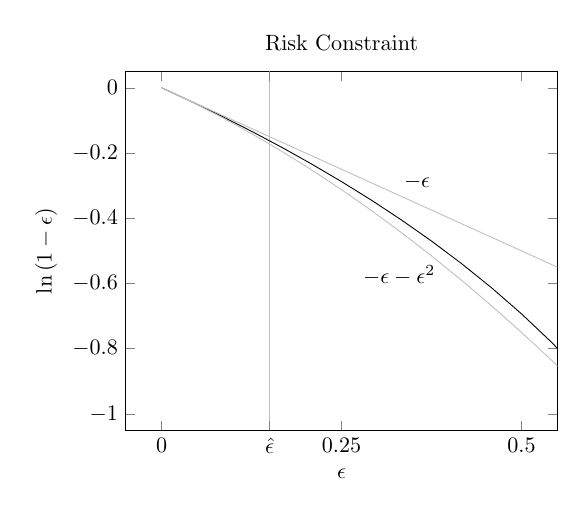
\begin{tikzpicture}[scale=.8]
\begin{axis}[ title=Risk Constraint,xlabel=$\epsilon$,ylabel=$\ln \left( 1-\epsilon \right)$,
  xmin=-.05,xmax=.55,
  ymin=-1.05,ymax=.05,
  xtick={0,.25,.5},
  	extra x ticks={.15},
	extra x tick style={grid=major},
	extra x tick labels={$\hat{\epsilon}$}
]
 \addplot[domain=0:.9999] { ln(1-x) };
 \addplot[domain=0:1,lightgray] {-x};
 \addplot[domain=0:1,lightgray] {-x - x^2};
  \node at (axis cs: .355,-.29) { $-\epsilon$};
  \node at (axis cs: .33,-.575) { $-\epsilon-\epsilon^2$};
\end{axis}
\end{tikzpicture}
\end{document}
